\renewcommand{\theequation}{\theenumi}
\renewcommand{\thefigure}{\theenumi}
\begin{enumerate}[label=\thesection.\arabic*.,ref=\thesection.\theenumi]
\numberwithin{equation}{enumi}
\numberwithin{figure}{enumi}
\numberwithin{table}{enumi}

\item Let X and Y be i.i.d random variables uniformly distributed on (0,4).Then \pr{X>Y|X<2Y} is
\begin{enumerate}
    \item 1/3
    \item 5/6
    \item 1/4
    \item 2/3
\end{enumerate}
\solution

The PDF is given by
\begin{align}
   &f_X (x)=f_Y (x)=\nonumber \begin{cases}
         \frac{1}{4}, &\text{if 0 \(< x <\) 4}\\
         0, &\text{otherwise}\\
   \end{cases} 
\end{align}    
The CDF is given by
\begin{align}
   \nonumber& F(x)=\int_{-\infty}^{x} f(x)dx \\ \nonumber
   &F_X (x)=F_Y (x)=\nonumber \begin{cases}
          0, & x\leq 0\\
         \frac{x}{4}, &\text{if 0 \(< x <\) 4}\\
          1, &x\geq4\\
   \end{cases}    
\end{align}
Using definition of conditional probability 
\begin{align}
    &\pr{X>Y|X<2Y}=\frac{\pr{Y < X< 2Y}}{\pr{X<2Y}} \label{eqn1}
\end{align}
Now finding \pr{X<2Y}
\begin{align}
    &\pr{X<2y}=F_X (2y)\\
    \implies& \pr{X<2Y}=\int_{-\infty}^{\infty} f_Y(x) \times F_X (2x)dx\\
    \implies& \pr{X<2Y}=\int_{0}^{2} \frac{x}{8}dx +\int_{2}^{4}\frac{1}{4}dx\\
    \implies& \pr{X<2Y}=\frac{3}{4}=0.75 \label{eqn2}
\end{align}
Now to find \pr{Y<X<2Y}
\begin{align}
    &\pr{y<X<2y}=F_X (2y)- F_X (y) \\
    \implies &\pr{Y<X<2Y}\\ \nonumber 
    &=\int_{-\infty}^{\infty} f_Y (x)( F_X (2x)- F_X(x))dx \\
   \implies &\int_{0}^{2}\frac{1}{4}\brak{\frac{x}{2}-\frac{x}{4}} dx +\int_{2}^{4}\frac{1}{4}\brak{1-\frac{x}{4}} dx\\
   \implies &\pr{Y<X<2Y}=\frac{1}{4}=0.25 \label{eqn3}
\end{align}
Now using \eqref{eqn1},\eqref{eqn2} and \eqref{eqn3}
\begin{align}
    \pr{X>Y|X<2Y}=\frac{1/4}{3/4}=\frac{1}{3}
\end{align}
Hence final solution is option 1) or 1/3 
%
\item Suppose $X$ is a positive random variable with the following probability density function,
\begin{align*}
f(x) = (\alpha x^{\alpha -1} + \beta x^{\beta-1} ) e^{-x^{\alpha}-x^{\beta}} ; x>0
\end{align*}
for $ \alpha >0, \beta >0$.
Then the hazard function of $X$ for some choices of $\alpha$ and $\beta$ can be
\begin{enumerate}
    \item an increasing function.
    \item a decreasing function.
    \item a constant function.
    \item a non monotonic function
\end{enumerate}
%
\solution


CDF of $X$, 
\begin{align}
    F(x) &=  \int_{-\infty}^xf(t)dt \\
    &= \int_{0}^xf(t)dt \hspace{1cm} \text{as } x>0\\
    &= \int_{-\infty}^t\left((\alpha t^{\alpha -1} + \beta t^{\beta-1} ) \times e^{-t^{\alpha}-t^{\beta}}\right)dt \\
    &= -e^{-t^{\alpha}-t^{\beta}} \Big|_0^x\\
    &= 1-e^{-x^{\alpha}-x^{\beta}}
\end{align}
Hazard function,
\begin{align}
    h(x) &= \frac{f(x)}{1-F(x)} \\
    &= \alpha x^{\alpha -1} + \beta x^{\beta-1} \\
    h^{\prime}(x) &= \alpha(\alpha -1) x^{\alpha -2} + \beta(\beta-1) x^{\beta-2}\\
     h^{\prime}(x) &= 
         \begin{cases}
    0 & \alpha=\beta=1 \\
    >0 & \text{otherwise}\\
    \end{cases}
    \end{align}
    Thus $h(x)$ can be either constant function or an increasing function.
    
    \begin{figure}[h]
    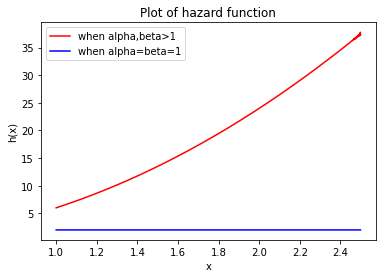
\includegraphics[width=\columnwidth]{solutions/2018/dec/118/figures/plot.png}
    \end{figure}
     From the above figure, it is verified that $h(x)$ can be either constant function or an increasing function.\\
       Correct options are 1,3.





%
\item Suppose n units are drawn from a population of N units sequentially as follows. A random sample
\begin{align}
    U_1, U_2, ... U_N \text{ of size N, drawn from }U\brak{0, 1} 
\end{align} 
The k-th population unit is selected if 
\begin{align}
    U_k<\frac{n - n_k}{N-k+1}, k = 1, 2, ..N. \text{where, } n_1=0, n_k = 
\end{align}
number of units selected out of first k-1 units for each k = 2, 3, ..N. Then,
\begin{enumerate}
    \item The probability of inclusion of the second unit in the sample
    \begin{align}
        \text{ is } \frac{n}{N}
    \end{align}
    \item The probability of inclusion of the first and the second unit in the sample
    \begin{align}
        \text{ is } \frac{n \brak{n-1}}{N \brak{N-1}}
    \end{align}
    \item The probability of not including the first and including the second unit in the sample
    \begin{align}
        \text{ is } \frac{n \brak{N-n}}{N \brak{N-1}}
    \end{align}
    \item The probability of including the first and not including the second unit in the sample
    \begin{align}
        \text{ is } \frac{n \brak{n-1}}{N \brak{N-1}}
    \end{align}
\end{enumerate}
%
\solution
\input{solutions/2018/dec/116.tex}

% \item Consider a Markov Chain with state space $\cbrak{0,1,2}$ and transition matrix
% \begin{align}
% P = 
% \begin{blockarray}{c@{\hspace{1pt}}rrr@{\hspace{3pt}}}
%          & 0   & 1   & 2 \\
%         \begin{block}{r@{\hspace{3pt}}@{\hspace{1pt}}
%     (@{\hspace{1pt}}rrr@{\hspace{1pt}}@{\hspace{1pt}})}
%         0 & \frac{1}{2} & \frac{1}{2} & 0  \\
%         1 & 0 &\frac{1}{2}  & \frac{3}{4}  \\
% %
%         2 &  \frac{1}{3} & \frac{1}{3} & \frac{1}{3}  \\
%         \end{block}
%     \end{blockarray}
% \end{align}
% For any two states $i$ and $j$, let $p_{ij}^{(n)}$ denote the $n$-step transition probability of going from $i$ to $j$.  Identify correct statements.
% \begin{enumerate}
% \item $\lim_{n \to \infty} p_{11}^{(n)} = \frac{2}{9}$
% \item $\lim_{n \to \infty} p_{21}^{(n)} = 0$
% \item $\lim_{n \to \infty} p_{32}^{(n)} = \frac{1}{3}$
% \item $\lim_{n \to \infty} p_{13}^{(n)} = \frac{1}{3}$
% \end{enumerate}
% \solution
% See Tables \ref{eq:solutions/2018/dec/106/table0} and \ref{eq:solutions/2018/dec/106/table1}


\onecolumn
	\begin{longtable}{|l|l|}
		\hline
		\multirow{3}{*}{Irreducible Markov Chain} 
		& \\
		& A Markov chain is $\textbf{irreducible}$ if all the states communicate with each other,\\
		& i.e., if there is only one communication class.\\
		&\\
		\hline
		\multirow{3}{*}{Aperiodic Markov Chain} & \\
		& If there is a self-transition in the chain ($p^{ii}>0$ for some i), then the chain is\\
		& called as $\textbf{aperiodic}$\\
		& \\
		\hline
		\multirow{3}{*}{Stationary Distribution} & \\
		& A stationary distribution of a Markov chain is a probability distribution that\\
		& remains unchanged in the Markov chain as time progresses. Typically, it is\\
		& represented as a row vector $\Vec{\pi}$ whose entries are probabilities summing to 1,\\ 
		& and given transition matrix $\textbf{P}$, it satisfies\\
		& \\
		&  \qquad \qquad  \qquad$\Vec{\pi} = \Vec{\pi} \textbf{P}$\\
		& \\
		\hline
\caption{}
\label{eq:solutions/2018/dec/106/table0}
	\end{longtable}
	\begin{longtable}{|l|l|}
		\hline
		\multirow{3}{*}{Drawing Transition diagram} 
		& \\
		& 
		
		$\begin{tikzpicture}[shorten >=1pt,node distance=2cm, scale =3, auto]
			\tikzstyle{every state}=[fill={rgb:black,1;white,10}]
			
			\node[state]   (q_1)                          {$1$};
			\node[state]   (q_2)  [right of=q_1]          {$2$};
			\node[state]   (q_3)  [below right of=q_1]          {$3$};
			
			\path[->]
			(q_1) edge [loop above] node {$\frac{1}{2}$}    (   )
			edge [bend left]  node {$\frac{1}{2}$}    (q_2)
			(q_2) edge [bend left]  node {$\frac{1}{2}$}    (q_3)
			edge [loop above] node {$\frac{1}{2}$}    ()
			(q_3) edge [bend left]  node {$\frac{1}{3}$}    (q_2)
			edge [bend left]  node {$\frac{1}{3}$}    (q_1)
			edge [loop below] node {$\frac{1}{3}$}    ();
		\end{tikzpicture}$
		
		\\  
		&\\
		&\\
		\hline
		\multirow{3}{*}{Checking whether the  } & \\
		& Here,\\chain is Irreducible
		& All the states are accessible to one another. \\and Aperiodic
		& $\implies$ They are in the same communication class. So, it is Irreducible.\\
		& \\
		& There exists the non- zero self-transition, which means that the chain \\
		& is Aperiodic.\\
		&\\ 
		& We know that if the Markov Chain is irreducible and aperiodic then \\
		& \qquad \qquad \qquad $\Vec{\pi}_{j} = \lim_{n \to \infty}P\{X_{n} = j\}$, $j = 1,...,N$ \\
		& These are the stationary probabilities. \\
		&\\
		\hline
		\multirow{3}{*}{Finding the Stationary} & \\
		& Stationary Probability can be represented as\\Probability Distributions
		& \qquad \qquad \qquad $\Vec{\pi} = \Vec{\pi} \vec{P}$\\
		& \\
		& \qquad $\implies$ $\myvec{v_{1}&&v_{2}&&v_{3}} = \myvec{v_{1}&&v_{2}&&v_{3}}\vec{P}$ \\
		& \\
		& Equating the above equation we get \\
		& \\
		& \qquad \qquad \qquad $\frac{1}{2}v_{1}-\frac{1}{3}v_{3} = 0$ $\label{eq:solutions/2018/dec/106/eq}$\\
		& \\
		& \qquad \qquad \qquad $\frac{1}{2}v_{1}-\frac{1}{2}v_{2} + \frac{1}{3}v_{3} = 0$\\
		& \\
		& \qquad \qquad \qquad $\frac{1}{2}v_{2}-\frac{2}{3}v_{3} = 0$\\
		& \\\
		& We see that summation of second and the third equation gives us the \\
		& first equation only. \\
		& And we know that the probability distribution will sum up to 1. \\
		& \\
		& \qquad \qquad \qquad $v_{1}+v_{2}+v_{3} = 1$ \\
		& \\
		& Therefore, we get the equation form as \\
		& \\
		& \qquad \qquad \qquad $\myvec{1&1&1\\\frac{1}{2}&0&\frac{-1}{3}\\\frac{1}{2}&\frac{-1}{2}&\frac{1}{3}}\myvec{v_{1}\\v_{2}\\v_{3}} = \myvec{1\\0\\0}$ \\
		& \\
		\hline
		\multirow{3}{*}{Solving the linear} & \\
		& The above linear equation can be solved using Gauss-Jordan method as\\equtions
		& \\
		& \qquad \qquad \qquad $\myvec{1&1&1&\vrule&1\\\frac{1}{2}&0&\frac{-1}{3}&\vrule&0\\\frac{1}{2}&\frac{-1}{2}&\frac{1}{3}&\vrule&0}$\\
		& \\
		& \qquad $\xleftrightarrow[]{R_2 \leftarrow R_2 - \frac{1}{2}R_1}$
		$\myvec{1&1&1&\vrule&1\\0&\frac{-1}{2}&\frac{-5}{6}&\vrule&\frac{-1}{2}\\\frac{1}{2}&\frac{-1}{2}&\frac{1}{3}&\vrule&0}$\\
		&\\
		& \qquad $\xleftrightarrow[]{R_3 \leftarrow R_3 - \frac{1}{2}R_1}$
		$\myvec{1&1&1&\vrule&1\\0&\frac{-1}{2}&\frac{-5}{6}&\vrule&\frac{-1}{2}\\0&-1&\frac{-1}{6}&\vrule&\frac{-1}{2}}$\\
		&\\
		& \qquad $\xleftrightarrow[]{R_2 \leftarrow \frac{-1}{2}R_2}$
		$\myvec{1&1&1&\vrule&1\\0&1&\frac{5}{3}&\vrule&1\\0&-1&\frac{-1}{6}&\vrule&\frac{-1}{2}}$\\
		&\\
		& \qquad $\xleftrightarrow[]{R_3 \leftarrow R_3 + R_2}$
		$\myvec{1&1&1&\vrule&1\\0&1&\frac{5}{3}&\vrule&1\\0&0&\frac{3}{2}&\vrule&\frac{1}{2}}$\\
		&\\
		& \qquad $\xleftrightarrow[]{R_3 \leftarrow \frac{3}{2}R_3}$
		$\myvec{1&1&1&\vrule&1\\0&1&\frac{5}{3}&\vrule&1\\0&0&1&\vrule&\frac{1}{3}}$\\
		&\\
		& \qquad $\xleftrightarrow[]{R_2 \leftarrow R_2 - \frac{5}{3}R_3}$
		$\myvec{1&1&1&\vrule&1\\0&1&0&\vrule&\frac{4}{9}\\0&0&1&\vrule&\frac{1}{3}}$\\
		&\\
		& \qquad $\xleftrightarrow[]{R_1 \leftarrow R_1 - R_3}$
		$\myvec{1&1&0&\vrule&\frac{2}{3}\\0&1&0&\vrule&\frac{4}{9}\\0&0&1&\vrule&\frac{1}{3}}$\\
		&\\
		& \qquad $\xleftrightarrow[]{R_1 \leftarrow R_1 - R_2}$
		$\myvec{1&0&0&\vrule&\frac{2}{9}\\0&1&0&\vrule&\frac{4}{9}\\0&0&1&\vrule&\frac{1}{3}}$\\
		&\\
		& $\therefore$, stationary probability distribution $\pi$ is given by \\
		& \qquad \qquad $\pi = \myvec{\frac{2}{9} & \frac{4}{9} & \frac{1}{3}}$ \\
		& \\
		\hline
		\multirow{3}{*}{Observations} & \\
		
		
		& Since the given transition probability matrix $\vec{P}$ is irreducible and aperiodic, \\
		& then $\lim_{n \to \infty} \vec{P}^{n}$ converges to a matrix with all rows identical and equal to $\vec{\pi}$. \\
		& \\
		& We were able to find $\vec{\pi}$ as $\myvec{\frac{2}{9} & \frac{4}{9} & \frac{1}{3}}$ \\
		& \\
		& $\lim_{n \to \infty} \vec{P}^{n} = \myvec{\frac{2}{9}&\frac{4}{9}&\frac{1}{3}\\\frac{2}{9}&\frac{4}{9}&\frac{1}{3}\\\frac{2}{9}&\frac{4}{9}&\frac{1}{3}}$\\
		& \\
		& From the above matrix, we get \\
		& \\
		& $\lim_{n \to \infty} \vec{P}^{n}_{11} = \frac{2}{9}$ \\
		&\\
		& $\lim_{n \to \infty} \vec{P}^{n}_{21} = \frac{2}{9}$ \\
		&\\
		& $\lim_{n \to \infty} \vec{P}^{n}_{32} = \frac{4}{9}$ \\
		&\\
		& $\lim_{n \to \infty} \vec{P}^{n}_{13} = \frac{1}{3}$ \\
		&\\
		\hline
		\multirow{3}{*}{Conclusion} & \\
		& From our observation we see that \\
		&\\
		& Options 1) and 4) are True.\\
		& \\
		\hline
\caption{}
\label{eq:solutions/2018/dec/106/table1}
	\end{longtable}
\twocolumn


\end{enumerate}
